\documentclass[
  captions=tableheading,
  bibliography=totoc, 
  titepage=firstiscover,
]{scrartcl}

\usepackage{blindtext} %neuer input

\usepackage{longtable} % Tabellen über mehrere Seiten

\usepackage[utf8]{inputenc} %neuer input

\usepackage{scrhack}

\usepackage[aux]{rerunfilecheck} %Warnung falls nochmal kompiliert werden muss

\usepackage{fontspec} %Fonteinstellungen

\recalctypearea{}

\usepackage[main=ngerman]{babel} %deutsche Spracheinstellung

\usepackage{ragged2e} %neuer input

\usepackage{amsmath, nccmath}

\usepackage{amssymb} %viele mathe Symbole

\usepackage{mathtools} %Erweiterungen für amsmath


\DeclarePairedDelimiter{\abs}{\lvert}{\rvert}
\DeclarePairedDelimiter{\norm}{\lVert}{\rVert}

\DeclarePairedDelimiter{\bra}{\langle}{\rvert}
\DeclarePairedDelimiter{\ket}{\lvert}{\rangle}

\DeclarePairedDelimiterX{\braket}[2]{\langle}{\rangle}{
#1 \delimsize| #2
}

\NewDocumentCommand \dif {m}
{
\mathinner{\symup{d} #1}
}


\usepackage[
  math-style=ISO,
  bold-style=ISO,
  sans-style=italic,
  nabla=upright,
  partial=upright,
  warnings-off={
    mathtools-colon,
    mathtools-overbracket,
  },
]{unicode-math}

\setmathfont{Latin Modern Math}
\setmathfont{XITS Math}[range={scr, bfscr}]
\setmathfont{XITS Math}[range={cal, bfcal}, StylisticSet=1]


\usepackage[
  locale=DE,
  separate-uncertainty=true,
  per-mode=reciprocal,
  output-decimal-marker={,},
]{siunitx}

\usepackage[autostyle]{csquotes} %richtige Anführungszeichen

\usepackage{xfrac}

\usepackage{float}

\floatplacement{figure}{htbp}

\floatplacement{table}{htbp}

\usepackage[ %floats innerhalb einer section halten
  section,   %floats innerhalb er section halten
  below,     %unterhalb der Section aber auf der selben Seite ist ok
]{placeins}

\usepackage[
  labelfont=bf,
  font=small,
  width=0.9\textwidth,
]{caption}

\usepackage{subcaption} %subfigure, subtable, subref

\usepackage{graphicx}

\usepackage{grffile}

\usepackage{booktabs}

\usepackage{microtype} %Verbesserungen am Schriftbild

\usepackage[
backend=biber,
]{biblatex}

\addbibresource{../lit.bib}

\usepackage[ %Hyperlinks im Dokument
  german,
  unicode,
  pdfusetitle,
  pdfcreator={},
  pdfproducer={},
]{hyperref}

\usepackage{bookmark}

\usepackage[shortcuts]{extdash}

%\usepackage{warpcol}


\begin{document}
    \title{ATP Übungsblatt 3}
    \author{  
    Tobias Rücker\\
    \texorpdfstring{\href{mailto:tobias.ruecker@tu-dortmund.de}{tobias.ruecker@tu-dortmund.de}
    \and}{,} 
    Paul Störbrock\\
    \texorpdfstring{\href{mailto:paul.stoerbrock@tu-dortmund.de}{paul.stoerbrock@tu-dortmund.de}}{}
    }
\maketitle
\center{\Large Abgabegruppe: \textbf{Mittw. 10-12 Uhr}}
\thispagestyle{empty}

\newpage
\tableofcontents
\thispagestyle{empty}
\newpage

\setcounter{page}{1}


\section{Aufgabe 7}

    \begin{figure}[H]
        \centering
        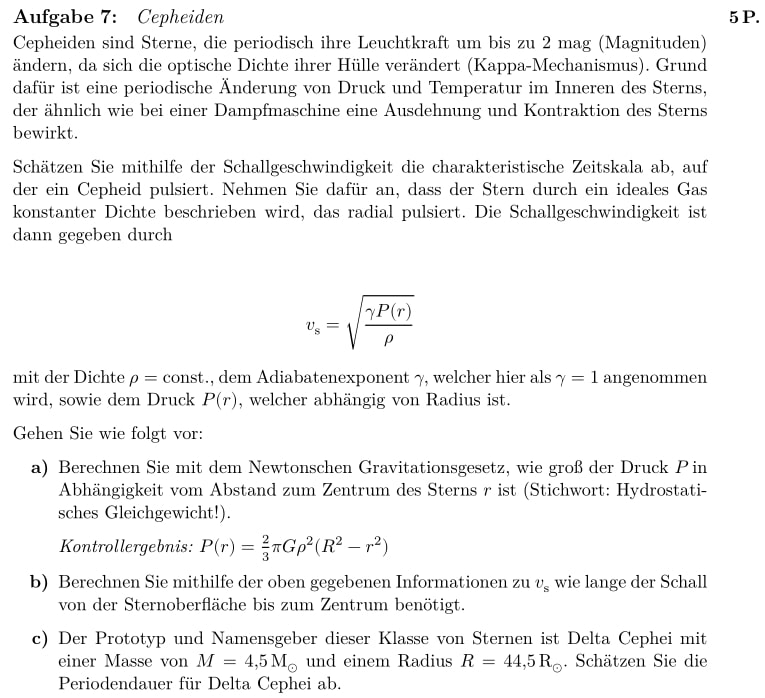
\includegraphics[width=\textwidth]{images/Aufgabe7abc.jpg}
        \label{fig:1}
    \end{figure}
    \begin{figure}[H]
        \centering
        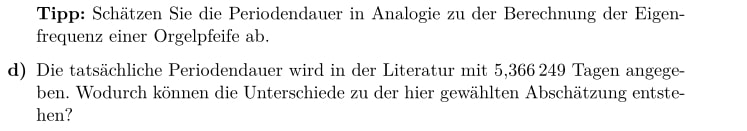
\includegraphics[width=\textwidth]{images/Aufgabe7d.jpg}
        \label{fig:2}
    \end{figure}

    \flushleft{\;}\justifying

\newpage
\subsection{a)}

Aus dem letzten Blatt:
\begin{align}
    \frac{GM \rho}{r^2}= \frac{\symup{d}p}{\symup{d}r}\\
    \intertext{
        Nebenrechnung:
    }
    M = \rho \cdot V\\
    = \rho \frac{4}{3} \pi r^3\\
    \intertext{
        Ende Nebenrechnung
    }
    -\frac{4}{3}\pi G \rho ^2 r = \frac{dP}{dr} \vert \int_r^R \symup{d} r'\\
    -\frac{4}{3}\pi G \rho ^2 \int_r^R r' \symup{d} r' = \int_r^R \frac{dP}{dr'} \symup{d} r'\\
    -\frac{2}{3} \pi  G \rho ^2 (R^2 -r^2) = \underbrace{P(R)}_{=0} -P(r)
    \intertext{
        Am Rand der Sonne wirkt keine Kraft wegen dem hydrostatischen Gleichgewicht, daher wird der Druck an der Stelle 0.
    } 
    P(r)=\frac{2}{3} \pi  G \rho ^2 (R^2 -r^2)
\end{align}


\subsection{b)}

\begin{align}
    v_s = \sqrt{\frac{\gamma P(r)}{\rho} }\\
    v_s = \sqrt{\frac{2}{3} \pi \gamma \rho G (R^2-r^2)}\\
    \gamma =1\\
    \frac{dr}{dt}= v_s\\
    dt = \frac{1}{v_s} dr \vert \int \\
    \int _0^t 1 dt = \int _0^R \sqrt{\frac{3}{2G \rho \pi}} \frac{1}{(R^2-r^2)^{\frac{1}{2}}} dr \\
    t= \int _0^R \sqrt{\frac{3}{2G \rho \pi}} \frac{1}{R\sqrt{1-\frac{r^2}{R^2}}} dr\\
    \intertext{
        Substitution
    }
    \frac{r}{R}=u\\
    \frac{du}{dr}=\frac{1}{R}\\
    dr = du R\\
    \intertext {
        Weiter
    }
    =\sqrt{\frac{3}{2G \rho \pi}} \int_0^1 \frac{1}{\sqrt{1-u^2}} du\\
    =\sqrt{\frac{3}{2G \rho \pi}} \arcsin(U) \vert_0^1 \\
    =\sqrt{\frac{3}{2G \rho \pi}} \frac{\pi}{2}
\end{align}



\subsection{c)}



\subsection{d)}

Die Abweichung in der Periodendauer kann daher stammen, dass der Stern als 
Zylinder angenähert wurde, wobei dieser mehr kugelförmig als zylinderförmig ist.

\section{Aufgabe 8}

\begin{figure}[H]
    \centering
    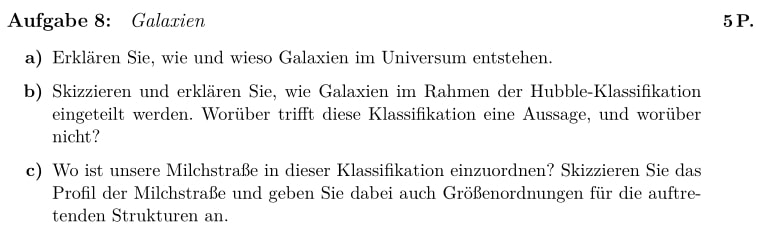
\includegraphics[width=\textwidth]{images/Aufgabe8.jpg}
    \label{fig:3}
\end{figure}

\newpage
\subsection{a)}

    \flushleft{Neue\;}\justifying Galaxien entstehen indem der dark-matter-halo Gas einfängt und dies auf das Zentrum der Galaxie lenkt. Im
    Inneren der Galaxie kühlt das Gas ab und bildet eine dünne Scheibe. Ist die Gasdichte groß genug, können sich Sterne bilden. Dies ist zum 
    Beispiel der Fall in den Spiralarmen unserer Milchstraße. Sobald die Galaxie groß genug ist, kann diese kleinere Galaxien einfangen und
    absorbieren, wodurch die Masse der Galaxie ansteigt. Im Laufe der Zeit sterben Sterne, wodurch mehr Materie in Form von Supernovae oder 
    planetarischen Nebeln der Galaxie beigefügt wird. Sterne der Population I befinden sich in der Regel auf der dünnen Scheibe der Galaxie, 
    wohingegen Sterne der Population II eher im Zentrum der Galaxie zu finden sind. Da Sterne aus Population II sehr alt und üblicherweise 
    in Kugelsternhaufen anzutreffen sind, und da die Sterndichte in Richtung Zentrum der Galaxie zunimmt, macht es durchaus Sinn, solche Sterne
    im Zentrum anzutreffen. 

    \flushleft{Der\;}\justifying Katalysator ist hier die Dunkle Materie. Obwohl sie nicht sichbar ist, ist die Wechselwirkung mit normaler Materie Messbar. Es wird vermutet, 
    dass jede Galaxie einen dark-matter-halo besitzt und in dem Frühstadium für den Materiezuwachs verantwortlich ist. Da das einfallende Gas
    jedoch nur Strahlungsenergie abgibt und den Drehimpuls beibehält, entstehen die dünne Scheibe und die Spiralarme, wie wir sie von unserer
    Milchstraße kennen. 

    \flushleft{Neben\;}\justifying Spiralgalaxien gibt es aber noch elliptische Galaxien. Diese gewinnen an Masse, indem sie mit anderen Galaxien verschmelzen. Innerhalb
    einer elliptischen Galaxie entstehen keine neuen Sterne mehr, da elliptische Galaxien sehr massereich sind und eine hohe Schwerkraft besitzen. 
    Unsere Milchstraße ist auf Kollisionskurs mit der Andromedagalaxie, was ebenfalls eine elliptische Galaxie zufolge haben kann.

\subsection{b)}

\begin{figure}[H]
    \centering
    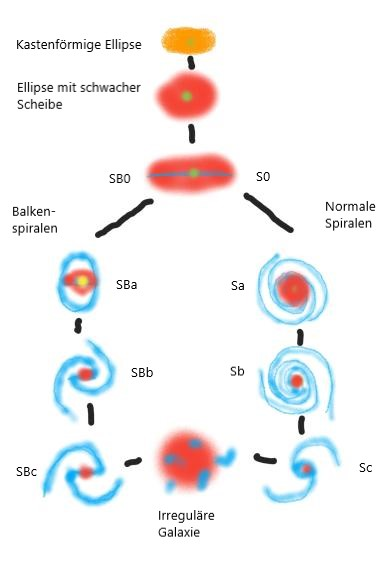
\includegraphics[width=0.75\textwidth]{images/Aufgabe8b_skizze.jpg}
    \label{fig:4}
\end{figure}

    \flushleft{Laut\;}\justifying Hubble beginnt jede Galaxie ihren Lebenszyklus als eine kastenförmige (E0) Galaxie. Diese gewinnt allmählich 
    an Form und wird über die nächsten zwei Stadien elliptischer, bis sie im Stadium S0/SB0 angelangt. Dort bildet die Galaxie die ersten 
    Anzeichen einer Scheibe, jedoch haben sich hier noch keine Arme geformt. 

    \flushleft{Im\;}\justifying Zweig der normalen Spiralen, wird zwischen der Lumiosität des Zentrums unterschieden, und wie eng die Spiralarme
    aneinander hängen. Eine Sa Galaxie zeichnet sich durch eine hohe Leuchtkraft und eng gewobenen Armen aus. Die Leuchtkraft und Enge der Arme 
    nimmt über Sb bis zu Sc ab. 

    \flushleft{Der\;}\justifying Balkenspiralenzweig ist die Klassifizierung ähnlich im Bezug auf normale Spiralen, da auch hier die Leuchtkraft
    und Enge der Spiralen zur Einteilung beitragen. Jedoch zeichnen sich Balkengalaxien sich durch den prominenten Balken aus, der sich durch das
    Zentrum der Galaxie zieht. Anders als bei Spiralgalaxien beginnt der Spiralarm nicht direkt im Zentrum, sondern etwas außerhalb. Der Balken
    besteht aus Sternen, die durch das Galaktische Zentrum hindurch gehen.

    \flushleft{Abschließend\;}\justifying gibt es noch irreguläre Galaxien. Diese werden in zwei Kategorien unterschieden. Irr I Galaxien sind 
    Galaxien, die trotz einer überwiegend unorganisierten Struktur dennoch ein wenig Ordnung vorweisen können (z.B. kleine Magellanische Wolken).
    Irr II Galaxien hingegen haben keine organisierte Struktur. 

    \flushleft{Hubble\;}\justifying erstellte dieses Ornungsschema als Leitfaden für das Alter einer Galaxie. Diese Annahme ist jedoch nicht korrekt.
    Außerdem trifft diese Klassifizierung keine Aussage über das Wechselwirken von Galaxien, z.B. wenn zwei Galaxien fusionieren. Die Galaxie Messier 82
    weist zwei Schwarze Löcher auf, welche eine hohe x-ray Emmissionsrate haben. Es ist noch nicht klar, ob die Schwarzen Löcher seit der Entstehung 
    der Galaxie existieren, oder später hinzugekommen sind. Aber es sind vielversprechende Kandidaten, um die Entstehung von Schwarzen Löchern zu
    untersuchen, die vergleichbar sind mit dem unserer Milchstraße (Sagittarius A*)



\subsection{c)}

\begin{figure}[H]
    \centering
    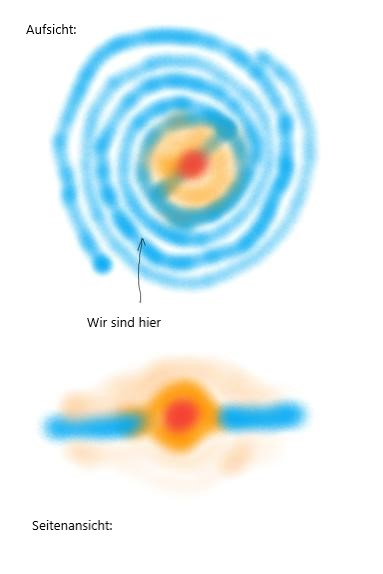
\includegraphics[width=0.75\textwidth]{images/Aufgabe8c_skizze.jpg}
    \label{fig:5}
\end{figure}

    \flushleft{Unsere\;}\justifying Milchstraße ist eine Balkenspiralgalaxie (SBb). Sie weist einen charakteristischen Balken im Zentrum vor und hat eng
    liegende Spiralarme. Der Balken hat eine Länge von ca. 15000 Lichtjahren.

    \flushleft{Der\;}\justifying Druchmesser unserer Milchstraße ist ca. 100000 Lichtjahre. Die Dicke der Scheibe (hier orange) ist ca. 3000
    Lichtjahre, nimmt aber im galaktischen Zentrum auf ca. 15000 Lichtjahre zu. Die Sonne befindet sich ca. 26000 Lichtjahre vom Zentrum der
    Milchstraße entfernt. 

\section{Aufgabe 9}

\begin{figure}[H]
    \centering
    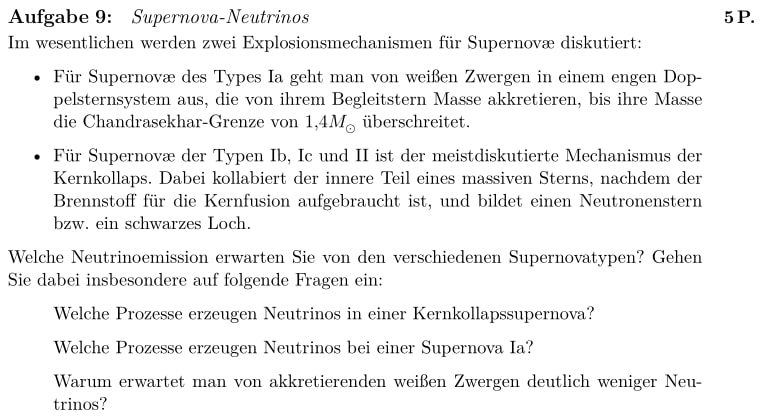
\includegraphics[width=\textwidth]{images/Aufgabe9.jpg}
    \label{fig:6}
\end{figure}

    \subsection{Kernkollapssupernova}

    \flushleft{Bei\;}\justifying einer Kernkollapssupernova ist eine Sternmasse von $M>1.4M_{\odot}$ vonnöten um den Entartungsdruck der Elektron,
    also das Chandrasekharlimit, zu überwinden. Diese Supernova wird auch als Supernova Typ II bezeichnet. Beim Kollaps des Kerns wird durch
    Photodesintegration das Eisen im Kern zu Helium gespalten, welches dann zu Protonen und Elektronen zerfällt. Anschließend zerfallen
    die Protonen und Elektronen durch inversen $\beta$-Zerfall zu Neutronen und Elektronneutrino:
    \begin{align*}
        p^+ + e^- &= n + \nu_e
    \end{align*}

    \subsection{Supernova Typ Ia}

    \flushleft{Bei\;}\justifying einer Supernova des Typs Ia entsteht, sobald ein weißer Zwerg Materie von einem roten Riesen akkretiert. 
    Dabei muss der weiße Zwerg hauptsächlich aus Sauerstoff und Kohlenstoff bestehen. Hat der weiße Zwerg genügend Masse und Temperatur
    (~Chandrasekharlimit), werden Sauerstoff und Kohlenstoff funsioniert. Dieser Prozess ist schlagartig (wenige Sekunden) und zerstört den
    Stern. Neutrinos werden hier hauptsächlich in den folgenden $\beta$-Zerfällen freigesetzt:
    \begin{align*}
        ^{56}\text{Ni} &\to ^{56}\text{Co} + e^+ + \nu_e\\
        ^{56}\text{Co} &\to ^{56}\text{Fe} + e^+ + \nu_e
    \end{align*}
    \flushleft{Hierbei\;}\justifying zerfällt $^{56}\text{Nickel}$ zu $^{56}\text{Cobalt}$, einem Proton und einem Elektronneutrino und $^{56}\text{Cobalt}$ zu $^{56}\text{Eisen}$, 
    einem Proton und einem Elektronneutrino.

    \subsection{Akkretierender weißer Zwerg $\to$ weniger Neutrinos?}

    \flushleft{Bei\;}\justifying einer Typ II Supernova zerfällt der gesamte Kern zu Neutronen und Neutrinos. Hierbei ist die Vorraussetzung, dass
    die Sternmasse vorher bei $M>1.4M_{\odot}$ liegt. Diese kann natürlich auch deutlich drüber liegen. Bei einem akkretierenden weißen Zwerg hingegen
    wird nur ein Teil der Teilchen fusioniert. Also entstehen bei Sternen gleicher Masse und unterschiedlichem Supernovatyps mehr Neutrinos 
    beim Typ II. Außerdem hat der akkretierende weiße Zwerg ~Chandrasekharmasse, was nach oben natürlich begrenzt ist. 

\end{document}
